% Author biographies and photos retained from the supplied author materials.

\begin{IEEEbiography}[{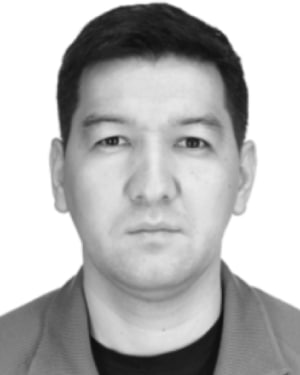
\includegraphics[width=1in,height=1.25in,clip,keepaspectratio]{author_photo_beibut_amirgaliyev.png}}]{Beibut Amirgaliyev}
(Member, IEEE) received the B.S. degree in information systems from Kazakh-British Technical University, and the M.S. degree in software engineering and the Ph.D. degree in computer science and mathematical modeling from the Kazakh National Technical University, Almaty, Kazakhstan. From 2010 to 2018, he was an Assistant Professor with International Information Technology University. Since 2019, he has been a Professor with the Department of Computer Engineering, Astana IT University. He has authored more than 40 papers indexed in Scopus and Web of Science. His research interests include smart city applications, machine learning, and innovation. He is Executive Editor of the Scientific Journal of Astana IT University.
\end{IEEEbiography}

\begin{IEEEbiography}[{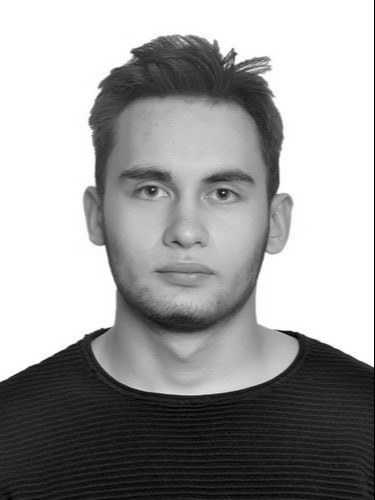
\includegraphics[width=1in,height=1.25in,clip,keepaspectratio]{author_photo_serzhan_ossenov.jpg}}]{Serzhan Ossenov}
(Member, IEEE) received the B.S. degree in Big Data Analysis from Astana IT University, Astana, Kazakhstan, in 2025. He is currently pursuing the M.S. degree in Applied Data Analytics at Astana IT University. Since 2026, he has been a Big Data Analyst with the National Bank of Kazakhstan, specializing in data quality and data governance. His research interests include privacy-preserving machine learning, image recognition, federated learning, differential privacy, and data quality.
\end{IEEEbiography}
